\section{Coding Progress}

\subsection*{Modifications to REM}

The most important modification to the original toolchain has been decoupling it
from the rust compiler. Previously, REM was heavily tied to rustc, the rust
compiler. It relied compiler specific representations of files and their syntax
trees. Because of this dependency, REM required a very specific buildchain, and
could not be used outside of this build context. Additionally, when I took over
the project, changes to external libraries meant that the toolchain was
completely non-functional. Some work is still required to bring the toolchain
off of nightly rust onto stable rust.\\
Additionally, REM’s data handling has been improved. The original approach
involved the three main components (controller, borrower, and repairer) passing
data via intermediary files. By restructuring data flow among the now five
modules, a 5-10\% speedup was achieved.

\subsection*{REM-Extract: Performing inital function extraction}

The REM-Extract tool is a drop in replacement for the initial code extraction
that REM used to rely on IntelliJ IDEA to perform. It is a pure Rust solution,
relying on RA to perform the code extraction, in preparation for the REM
toolchain to be integrated into RA at a later date. At the highest level of
abstraction, the extractor performs two tasks:

\begin{enumerate}
    \item Extracting the function from the source code (i.e. directly copying
    the users selected code into a new function).
    \item Inferring the types of the variables in the function, and adding them
    to the function signature, as well as annotating the caller with the correct
    variables. Type inference is the ``compile-time process of reconstructing
    missing type information in a program'' \cite{DUGGAN199637}. Because of
    Rust's very strict type system, this is a far more complex task than in a
    dynamically typed languages like Python or Ruby.
\end{enumerate}

Extracting the function becomes an exponentially more complex task as the more
complex language features of Rust are used. In the below example, the extraction
of \textit{extracted\_fn} is relatively trivial, but demonstrates the basic
principles of the extraction tool.

{\small
\inputminted[linenos, tabsize=4]{rust}{snippets/simple_extract.rs}}

Appenix \ref{app:goal} contains a more complex example of a function
that the toolchain is working towards supporting.

The graph below depicts the development progress of the
extraction tool over the last 5 weeks. The tool will continue to be developed as
the capabilities of the toolchain are expanded. Most of the test failures at
this point are for the reasons outlined in section 5.1.

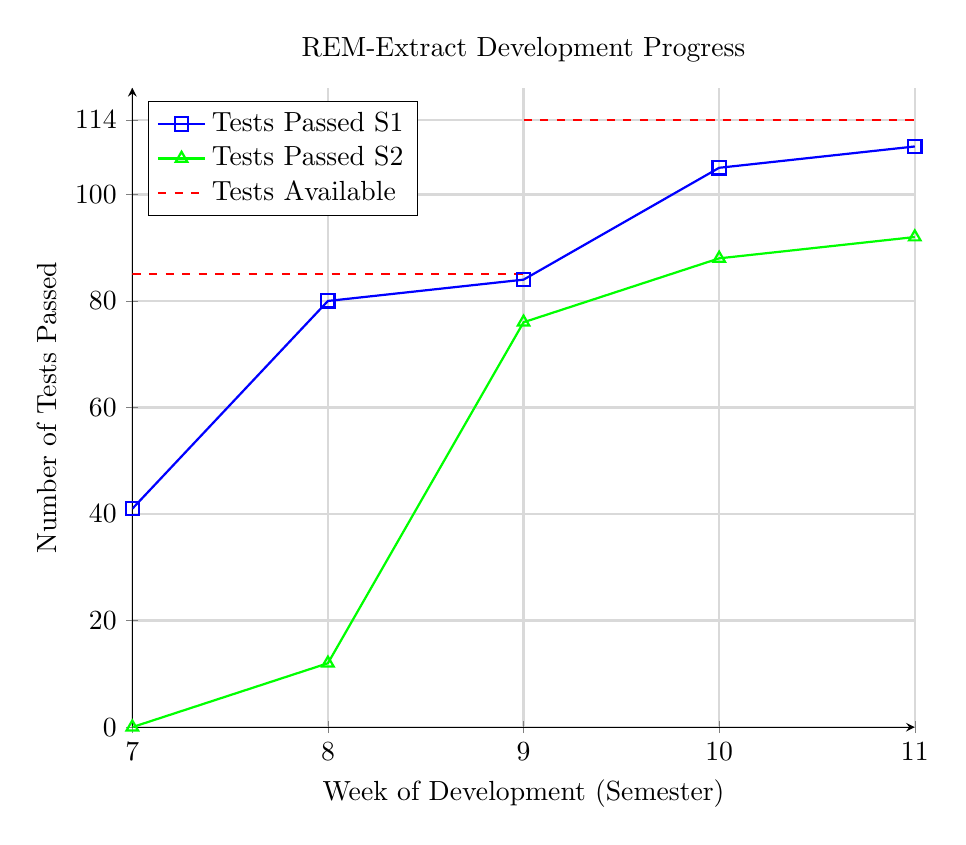
\begin{tikzpicture}\label{graph:rem-extract}
    \centering
    \begin{axis}[
        width=0.95\columnwidth,
        height=0.8\columnwidth,
        title={REM-Extract Development Progress},
        xlabel={Week of Development (Semester)},
        ylabel={Number of Tests Passed},
        xmin=7, xmax=11,
        ymin=0, ymax=120,
        xtick={7, 8, 9, 10, 11},
        ytick={0, 20, 40, 60, 80, 100, 114},
        grid=both,
        major grid style={line width=0.8pt,draw=gray!30},
        minor grid style={draw=gray!15},
        legend style={
            at={(0.02,0.98)},
            anchor=north west,
            legend cell align=left,
            draw=black,
        },
        axis lines=left,
        ymajorgrids=true,
        xmajorgrids=true,
        every axis plot/.append style={thick}
    ]

    % Plot data
    \addplot[
        color=blue,
        mark=square,
        mark options={scale=1.2, fill=blue},
    ]
    coordinates {
        (7, 41)
        (8, 80)
        (9, 84)
        (10, 105)
        (11, 109)
    };
    \addlegendentry{Tests Passed S1}

    \addplot[
        color=green,
        mark=triangle,
        mark options={scale=1.2, fill=green},
    ]
    coordinates{
        (7, 0)
        (8, 12)
        (9, 76)
        (10, 88)
        (11, 92)
    };
    \addlegendentry{Tests Passed S2}

    % Line indicating the total number of tests available
    \addplot[
        color=red,
        dashed,
        domain=7:9,
    ]
    {85};
    \addplot[
        color=red,
        dashed,
        domain=9:11,
    ]
    {114};
    \addlegendentry{Tests Available}

    \end{axis}
\end{tikzpicture}

\subsection*{REM-CLI: A comprehensive command line interface for REM}

The REM-CLI provides a unified interface for developers to interact with the
5 separate modules of REM. It streamlines the process of performing method
extraction by offering an intuitive command-line interface that handles
everything from code analysis to extraction. By consolidating the toolchain into
a single, easy-to-use CLI, REM removes the need for users to manually manage
multiple stages of the extraction process. It is also needed to itegrate the
functionality into a code editor.

\subsection*{REM-VSCode: A Visual Studio Code extension for REM}

The REM-VSCode extension is a proof of concept that demonstrates how the REM
tool can be easily integrated into any code editor. It provides a user-friendly interface
within the far more popular Visual Studio Code editor. Because the entire
backend of REM is now written in Rust, the extension is able to be independent
of a specific platform, and thanks the the previous work on decoupling the tool
from rustc, it no longer requires a very specific environment / buildchain to
run. It is available on the
\href{https://marketplace.visualstudio.com/items?itemName=MatthewBritton.remvscode&ssr=false#overview}{VSCode
Marketplace}, but isn't finalised yet.